%% Copernicus Publications Manuscript Preparation Template for LaTeX Submissions
%% ---------------------------------
%% This template should be used for the following class files: copernicus.cls, copernicus2.cls, copernicus_discussions.cls
%% The class files, the Copernicus LaTeX Manual with detailed explanations regarding the comments
%% and some style files are bundled in the Copernicus Latex Package which can be downloaded from the different journal webpages.
%% For further assistance please contact the Publication Production Office (production@copernicus.org).
%% http://publications.copernicus.org


%% Differing comments regarding the specific class files are highlighted.


%% copernicus.cls
\documentclass[acp]{copernicus}

%% copernicus2.cls
%\documentclass[acp]{copernicus2}

%% copernicus_discussions.cls
%\documentclass[journal abbreviation, hvmath, online]{copernicus_discussions}


\begin{document}


\title{Something about cloud tracking}


\author[1]{Jordan T Dawe}
\author[1]{Philip H Austin}

\affil[1]{Department of Earth and Ocean Sciences, 
        University of British Columbia, 
	6339 Stores Road, 
        Vancouver, BC, 
        V6T 1Z4}

%% The [] brackets identify the author to the corresponding affiliation, 1, 2, 3, etc. should be inserted.



\runningtitle{CLOUD TRACKING}

\runningauthor{Dawe and Austin}

\correspondence{Jordan T Dawe\\ (jdawe@eos.ubc.ca)}



\received{}
\pubdiscuss{} %% only important for two-stage journals
\revised{}
\accepted{}
\published{}

%% These dates will be inserted by the Publication Production Office during the typesetting process.


\firstpage{1}

\maketitle



\begin{abstract}
A technique for the tracking of individual clouds in an large eddy 
simulation model is presented.
\end{abstract}


%% only used for copernicus2.cls
%\abstract{
% TEXT
% \keywords{TEXT}}



\introduction
%% \introduction[modified heading if necessary]
TEXT



\section{Model Description}

All LES calculations in this paper were made using the System for Atmospheric 
Modeling \citep[SAM;][]{Khairoutdinov2003}.  SAM is an anelastic LES 

Two model runs were performed, configured as standard Global Energy and Water
Cycle Experiment (GEWEX) Cloud System Studies \citep[GCSS;][]{Randall2003}
experiments: a Barbados Oceanographic and Meteorological Experiment 
\citep[BOMEX;][]{Siebesma2003} run, and an Atmospheric Radiation Measurement
Study \citep[ARM;][]{Brown2002} run. 

\subsection{BOMEX}

BOMEX simulates a trade-wind cumulus cloud field observed over ocean near 
Bermuda

The BOMEX run was performed on a 6.4 km x 6.4 km horizontal x 3.2 km vertical 
domain with 25 meter grid resolution in all directions for 6 hours, and the 
first three hours of simulation were discarded. 

\subsection{ARM}

The ARM run was performed on a 7.68 km x 7.68 km x 4.5 km domain with 30 meter 
grid resolution.


%==============================================================================

\section{Cloud Tracking}

Dividing a cloud field up into individual clouds at a single moment in time is 
a trivial matter of finding connected cloudy regions.  Tracking the resulting 
clouds from one time step to the next is more problematic, as a cloud is not a 
consistent physical object.  It is, rather, a series of processes: A rising 
parcel of moist air may condense, a parcel of air containing condensate may 
evaporate, and a cloud may merge with another cloud or split into multiple 
clouds.  To be able to handle all of these processes, we adopt a more complex 
definition of what constitutes an individual cloud.

We begin by defining two cloud regions.  First is the cloud core, defined 
following \cite{Siebesma1995} as all cloudy points which have positive 
buoyancy and upward velocity.  Second is the cloud plume, the region of air 
that is moving upward due to the cloud.  We define this region following the 
work of \cite{Couvreaux2010} via a numerical tracer that is emitted at the 
surface and subsequently decays exponentially with a one minute time constant.  
A point is considered to be in the plume if the tracer value of that point is 
larger than one standard deviation above the mean tracer value at the current 
model height.  Additionally, the tracer must exceed five precent of the value 
of the tracer standard deviation integrated from the surface to the current 
height.  Unlike Couvreaux et al., we do not require upper-level plume points 
to have condensed liquid water.  Finally, we force the core region to be a 
subset of the plume by setting all core points to also be plume points.

Next, we divide the cloud field into ``cloudlets" by assigning any core points 
which are nearest-neighbour adjacent to the same cloudlet.  These core 
cloudlets are then expanded into nearest-neighbour connected plume points 
until all plume points that are connected to a core are assigned to a 
cloudlet.  Remaining plume points are then divided into plume cloudlets which 
have no cores.  This process is repeated for every saved model time step.

These cloudlets are then assigned to belong to clouds.  For the first time step,
we simply assign each cloudlet to a seperate cloud.  At subsequent time steps,
cloudlets that spatially overlap with a cloud at the previous timestep are
assumed to be the same cloud.  The cloudlet's position is corrected for
advection using the mean velocity of the cloudlet's core (if core points are
present in the cloudlet) or plume (if they are not), multiplied by the time
between model output saves.

Four kinds of overlap are possible: core points in the cloudlet may overlap 
core points in a previous time step cloud (core-core); cloudlet core may 
overlap plume points (core-plume); plume may overlap core (plume-core); and 
plume may overlap plume (plume-plume).  Several kinds of overlap may occur 
simultaneously, so we define a heirarchy of connection types and check each 
in turn.  The strongest connection type is core-core, followed by core-plume,
then plume-plume.  Plume-core connections are ignored, which prevents 
connections between newly formed core cloudlets and leftover plume from 
a dissipating cloud.  Conversely, allowing core-plume connections lets us 
associate newly created cloud cores with plumes rising through the sub-cloud 
layer.  Only the strongest connection type present for a given cloudlet is 
considered: if a cloudlet has core-core connections, any core-plume or 
plume-plume connections are ignored, and if there are core-plume connections,
plume-plume connections are ignored.  Finally, a cloudlet may connect to more
than one cloud, which is used to identify merges and splits.

Any cloudlet which overlaps more than one previous time step cloud is 
considered to be the result of a merge between the two clouds.  In this case 
the cloudlet is assigned to the cloud with the largest overlap, and the 
other overlapping clouds are assumed to have merged with the largest overlap
cloud.  Next, clouds that connect to more than one cloudlet are considered for
splitting.  Splits occur only if a cloud contains more than one cloudlet whose
plume is in contact with the ground, with the largest cloudlet being assigned 
to the original cloud and the smaller sub-clouds becoming new clouds. 
Cloudlets which are not connected to the ground are assigned to the nearest
ground-connected cloudlet, measured from the centroids of the cloudlets.  
Any cloudlets that do not overlap clouds in the previous time step are assumed
to be new clouds.  This process of cloudlet assignment, merging, splitting, and 
creation is repeated for each time step until all cloudlets are assigned to a
cloud.
  
Once the cloudlets are all assigned to a cloud, any cloud that has cloud core points for less than five minutes is flagged as noise.  If any merge or split 
events occured over these clouds' short lifetimes, the noise cloud is rejoined 
to the cloud it split from or merged into.  This prevents clouds that split
then immediately re-merge with their parent cloud, and decaying cloud detritus 
above cloudbase, from being counted as discrete cloud objects.  Remaining 
noise clouds are separated from the main cloud database and considered to be a mixture of ``mistakes" in the tracking algorithm and short-lived, dynamically forced clouds at cloud base.

%==============================================================================

\section{Tracked Cloud Statistics}

First we examine the population statistics of the tracked cloud ensembles we 
have isolated with our tracking algorithm for the BOMEX and ARM GCSS cases.

\subsection{BOMEX}

Over the 3 hour BOMEX run

\subsection{ARM}

TEXT

%==============================================================================

\section{Cloud Initiation}
TEXT

\subsection{BOMEX}
TEXT

\subsection{ARM}
TEXT

\conclusions
%% \conclusions[modified heading if necessary]
TEXT




%\appendix
%\section{\\ \\ \hspace*{-7mm} HEADING}    %% Appendix A

%\subsection                               %% Appendix A1, A2, etc.




\begin{acknowledgements}
Support for this research was provided by the Canadian Foundation for Climate 
and Atmospheric Science through the Cloud Aerosol Feedback and Climate 
network.  Figures were generated using the matplotlib library in the Python
programming language.
\end{acknowledgements}


\bibliographystyle{copernicus}
\bibliography{./bibliography/cloud_tracking}


%% Literature citations
%% command                        & example result
%% \citet{jones90}|               & Jones et al.\ (1990)
%% \citep{jones90}|               & (Jones et al., 1990)
%% \citep{jones90,jones93}|       & (Jones et al., 1990, 1993)
%% \citep[p.~32]{jones90}|        & (Jones et al., 1990, p.~32)
%% \citep[e.g.,][]{jones90}|      & (e.g., Jones et al., 1990)
%% \citep[e.g.,][p.~32]{jones90}| & (e.g., Jones et al., 1990, p.~32)
%% \citeauthor{jones90}|          & Jones et al.
%% \citeyear{jones90}|            & 1990






%% FIGURES %%%%%%%%%%%%%%%%%%%%%%%%%%%%%%%%%%%%%%%%%%%%%%%%%%%%%%%%%%%%%%%%%%%%


%% ONE-COLUMN FIGURES

%f
%\begin{figure}[t]
%\vspace*{2mm}
%\begin{center}
%\includegraphics[width=8.3cm]{./figures/figure1}
%\end{center}
%\caption{Schematic representation of our cloudlet algorithm.}
%\label{fig:cloudfinder_instructions}
%\end{figure}


%% TWO-COLUMN FIGURES

%f
\begin{figure*}[t]
\vspace*{2mm}
\begin{center}
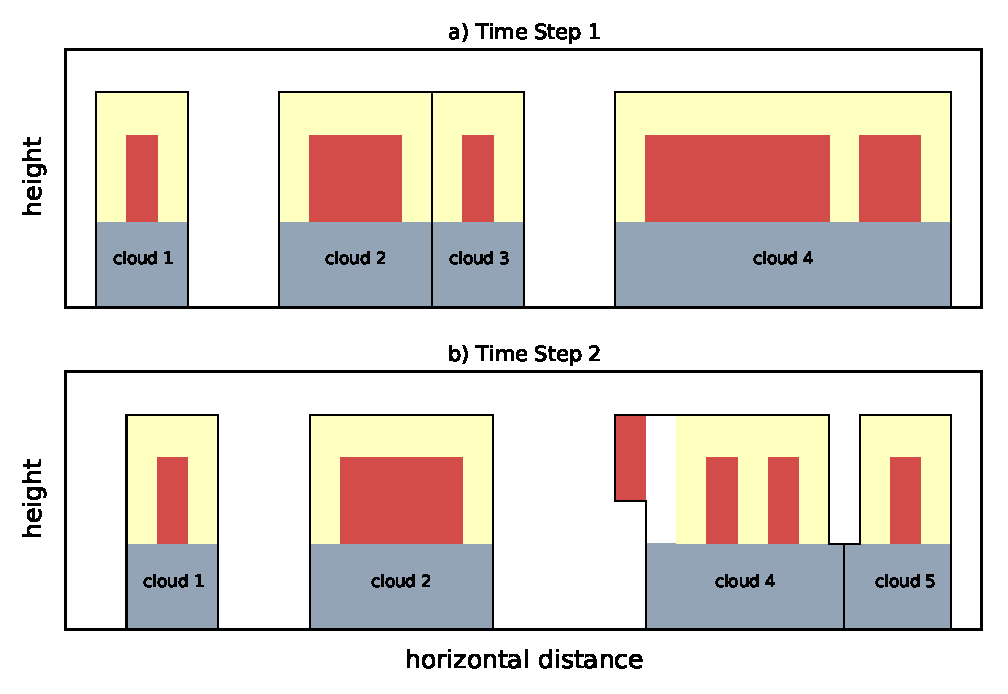
\includegraphics[width=\textwidth]{./figures/cloudfinder_instructions}
\end{center}
\caption{Schematic representation of our cloud tracking algorithm.}
\label{fig:cloudfinder_instructions}
\end{figure*}


%% TABLES %%%%%%%%%%%%%%%%%%%%%%%%%%%%%%%%%%%%%%%%%%%%%%%%%%%%%%%%%%%%%%%%%%%%


%% ONE-COLUMN TABLE

%t
\begin{table}[t]
\caption{Lifecycle statistics of tracked clouds}
\vskip4mm
\centering
\begin{tabular}{llcr}
\tophline
&&BOMEX&ARM\\
\middlehline
Total Clouds&&1183&1320\\
Starts\\
&Broken&59&n/a\\
&Split&339&319\\
&New&785&1001\\
Ends\\
&Broken&39&n/a\\
&Merge&51&61\\
&Decay&1093&1259\\

\bottomhline
\end{tabular}
\end{table}


%% TWO-COLUMN TABLE

%t
%\begin{table*}[t]
%\caption{TEXT}
%\vskip4mm
%\centering
%\begin{tabular}{column = lcr}
%\tophline

%\middlehline

%\bottomhline
%\end{tabular}
%\end{table*}


%% The different columns must be seperated with a & command and should
%% end with \\ to identify the column brake.

%%%%%%%%%%%%%%%%%%%%%%%%%%%%%%%%%%%%%%%%%%%%%%%%%%%%%%%%%%%%%%%%%%%%%%%%%%%%%%


%% If figures and tables must be numbered 1a, 1b, etc. the following command
%% should be inserted before the begin{} command.

%\addtocounter{figure}{-1}\renewcommand{\thefigure}{\arabic{figure}a}


\end{document}
